\documentclass[aspectratio=169, ignorenonframetext]{beamer}
\usepackage{pgf}

\mode<article>{
  \usepackage{fullpage}

}

\mode<presentation>
{
%   \usetheme{Madrid}
%   \useinnertheme{circles}
  \setbeamertemplate{navigation symbols}{}
%   \usetheme[hideothersubsections, width=2.4cm]{Hannover}
%   \usetheme{Antibes}
%   \usetheme{Montpellier}
  \usetheme{Singapore}
%   \usecolortheme{seahorse}
   \setbeamertemplate{footline}
   {%
%      \begin{beamercolorbox}{section in head/foot}
%       \usebeamercolor{bg}
       \hskip 1em \footnotesize \insertframenumber{} / \inserttotalframenumber%\hskip 41em \includegraphics[height = .5cm]{../../../../bilder/cc_by-nc_eu.png}
% % cc_by-nc_eu.png: 403x141 px, 72dpi, 14.22x4.97 cm, bb=0 0 403 141
%
% % bwslogo_3.png: 476x392 px, 300dpi, 4.03x3.32 cm, bb=0 0 114 94
%
%       %\hskip 5em
%       %       \input{../bilder/cc_by.png}
%       %\includegraphics[height=.5cm]{../../../../bilder/bwslogo_3.png}
%      \end{beamercolorbox}%
   }
  \usepackage{beamerfoils}
}
\usepackage[german]{babel}
\usepackage[utf8]{inputenc}
\usepackage{times}
\usepackage[T1]{fontenc}
\usepackage{eurosym}
\usepackage{graphicx}
\usepackage{amsmath}
\usepackage[siunitx,european]{circuitikz}
\usepackage{ulem}
\usepackage{listings}
%
\lstset{numbers=left, numberstyle=\tiny, stepnumber=2, numbersep=5pt, language = C++, alsolanguage=XML}
% \MyLogo{\includegraphics[height=1cm]{../../../../bilder/bwslogo_3.png}}
% % \includegraphics{../../bilder/bwslogo_3.png}
% % bwslogo_3.png: 476x392 px, 300dpi, 4.03x3.32 cm, bb=
%
\only<article>{
  \usepackage[colorlinks=true,linkcolor=blue,filecolor=magenta,urlcolor=cyan]{hyperref}
}

\only<presentation>{
  \usepackage{hyperref}
}


\title{Maschenstromverfahren / Kreisstromverfahren}
\subtitle{"`Schaltung 5"' Ersatzmodell für einen Transistor in Emiterschaltung}
% \date{V 0.2.0 - im Aufbau\\ Stand: \today}%\\

\institute[BWS Hofheim]{Brühlwiesenschule, Hofheim}
\author{Thomas Maul}

\titlegraphic{Für eigene Teile gilt: \includegraphics[height=1cm]{cc_by-nc_eu.png}}

\begin{document}
%   \only<article>{
%     \maketitle
%     \tableofcontents
%     \clearpage
%   }
\begin{frame}<beamer>
  \titlepage
  % \hyperlink{Teil_2}{\beamerbutton{Go part 2}}
\end{frame}

\begin{frame}
    \frametitle{Inhalt}
    \tableofcontents
  \end{frame}


\section{Aufgabe}
\begin{frame}{Aufgabenstellung}
\begin{figure}
 \includegraphics{schaltung5_transistor_emiterschaltung/schaltung5_0.png}
 \label{abb:Schaltung5_1Basis}
\end{figure}
\end{frame}

\begin{frame}{Knoten}
\begin{figure}
 \includegraphics{schaltung5_transistor_emiterschaltung/schaltung5_1knoten.png}
 \label{abb:Schaltung5_2knoten}
\end{figure}
\end{frame}

% \section{Transistor - Ersatzmodell}
\begin{frame}{Transistor als Ersatzmodell}
\begin{figure}
 \includegraphics{schaltung5_transistor_emiterschaltung/schaltung5_2transistor.png}
 \label{abb:Schaltung5_3transistor}
\end{figure}
\end{frame}

% \section{Ströme in der Schaltung}
\begin{frame}{Ströme in der Schaltung}
\begin{figure}
 \includegraphics{schaltung5_transistor_emiterschaltung/schaltung5_3stroeme.png}
 \label{abb:Schaltung5_3stroeme}
\end{figure}

Aufgabe:

\begin{itemize}
 \item Zeichne den vollständigen Baum einen.
 \item Lege die Maschen und Umlaufrichtung fest.
 \item Stelle das Gleichungssystem für die Maschenströme Aufbau.
 \item berechne die Maschenströme und die übrigen Ströme der Schaltung.
\end{itemize}
\end{frame}

\begin{frame}{Ergebnis der Simulation}
\begin{figure}
 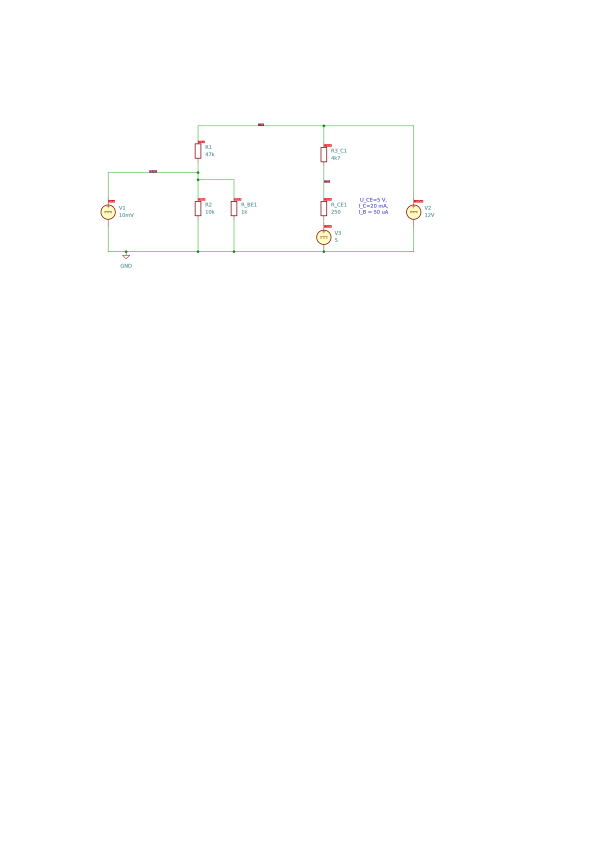
\includegraphics[scale = 1.3]{schaltung5_transistor_emiterschaltung/schaltung5_simu.png}
 % schaltung5_simu.png: 334x144 px, 96dpi, 8.84x3.81 cm, bb=
 \caption{Ergebnis der Simulation - Schaltung liegt als KICad-Datei in Github}
 \label{abb:Schatung5Simu}
\end{figure}
\end{frame}

\section{Einzelschritte}
\begin{frame}{Quelle umwandeln}
 \begin{figure}
 \includegraphics{schaltung5_transistor_emiterschaltung/schaltung5_4quelleUmgewandelt.png}
 % schaltung5_4quelleUmgewandelt.png: 1087x473 px, 300dpi, 9.20x4.00 cm, bb=0 0 261 114
 \label{abb:schaltung5_4quelleUmgewandelt}
\end{figure}

\end{frame}

\begin{frame}{vollständigen Baum einzeichnen}
 \begin{figure}
 \includegraphics{schaltung5_transistor_emiterschaltung/schaltung5_5baum.png}
 \label{abb:Baum}
\end{figure}
\end{frame}

\begin{frame}{Maschen einzeichnen\\Masche 1}
  \begin{figure}
 \includegraphics{schaltung5_transistor_emiterschaltung/schaltung5_5masche1.png}
 \label{abb:Schaltung5_masche1}
\end{figure}
\end{frame}

\begin{frame}{Maschen einzeichnen\\Masche 2}
  \begin{figure}
  \includegraphics{schaltung5_transistor_emiterschaltung/schaltung5_5masche2.png}
    \label{abb:Schaltung5_masche2}
\end{figure}
\end{frame}

\begin{frame}{Maschen einzeichnen\\Masche 3}
  \begin{figure}
 \includegraphics{schaltung5_transistor_emiterschaltung/schaltung5_5masche3.png}
 \label{abb:Schaltung5_masche3}
\end{figure}
\end{frame}

\begin{frame}{Maschen einzeichnen\\Masche 4}
  \begin{figure}
 \includegraphics{schaltung5_transistor_emiterschaltung/schaltung5_5masche4.png}
 \label{abb:Schaltung5_masche4}
\end{figure}
\end{frame}

\begin{frame}{Gleichungssystem I}
  \begin{figure}
 \includegraphics{schaltung5_transistor_emiterschaltung/schaltung5_5masche4.png}
 \label{abb:Schaltung5_masche4_wdh}
\end{figure}

\[
\left(
\begin{array}{cccc}
  R_2&&&\\
  &R_2+r_{be}&&\\
  &&R_2+R_1+R_{3C}+r_{ce}&\\
  &&&R_1+R_2
\end{array}
\right) \cdot
\left(
\begin{array}{c}
  I_{M1}\\I_{M2}\\I_{M3}\\I_{M4}
\end{array}
\right)=
\left(
\begin{array}{c}
  U_{q1}\\
  0\\
  -U_{q3}\\
  U_{q2}
\end{array}
\right)
\]
\end{frame}

\begin{frame}{Gleichungssystem II}
  \begin{figure}
 \includegraphics{schaltung5_transistor_emiterschaltung/schaltung5_5masche4.png}
 \label{abb:Schaltung5_masche4_wdh2}
\end{figure}

\[
\left(
\begin{array}{cccc}
  R_2&-R_2&-R_2&R_2\\
  -R_2&R_2+r_{be}&R_2&-R_2\\
  -R_2&R_2&R_2+R_1+R_{3C}+r_{ce}&-R_2-R_1\\
  R_2&-R_2&-R_2-R_1&R_1+R_2
\end{array}
\right) \cdot
\left(
\begin{array}{c}
  I_{M1}\\I_{M2}\\I_{M3}\\I_{M4}
\end{array}
\right)=
\left(
\begin{array}{c}
  U_{q1}\\
  0\\
  -U_{q3}\\
  U_{q2}
\end{array}
\right)
\]
\end{frame}

\begin{frame}{Gleichungssystem III}
  \begin{figure}
 \includegraphics{schaltung5_transistor_emiterschaltung/schaltung5_5masche4.png}
 \label{abb:Schaltung5_masche4_wdh3}
\end{figure}

\[
\left(
\begin{array}{cccc}
  10\,k&-10\,k&-10\,k&10\,k\\
  -10\,k&11\,k&10\,k&-10\,k\\
  -10\,k&10\,k&61,95\,k&-57\,k\\
  10\,k&-10\,k&-57\,k&57\,k
\end{array}
\right) \cdot
\left(
\begin{array}{c}
  I_{M1}\\I_{M2}\\I_{M3}\\I_{M4}
\end{array}
\right)=
\left(
\begin{array}{c}
  10\ mV\\
  0\\
  -5\,V\\
  12\,V
\end{array}
\right)
\]
\end{frame}

\label{lastpage}
\end{document}


